
\section{Travel to Valboro}

\begin{multicols*}{2}
	
Upon agreeing to escort Farzaren to Valboro, the adventurers are expected to meet Farzaren at the docks to board a medium-sized sail-ship for the trip. The crew consists of Farzaren, the ship’s captain (Half-Orc Elf named Alkath), and four deckhands (Gibnor, Tobferd, Radlael, Occar). The ship’s cargo consist of gold (heavily guarded), fabrics, materials, various tools, equipment, food and water. The ship’s crew is not well trained in combat, therefore, in the face of any threat, they will prefer to negotiate a way out or hide. The adventurers will be expected to handle any security concerns encountered on the voyage there.\break

\colorbox{pink}{\begin{minipage}{0.4\textwidth}
\subsubsection*{Role Playing Farzaren}
\begin{itemize}
	\item Farzaren is a flamboyant and generous wealthy noble. Since most of his wealth has been inherited from his family's business, he can come across as a spoiled brat, but is still generally friendly. 
	\item Farzaren cowers away from fights, and knows very little about anything other than commerce, specifically his family's wine business.
	\item Farzaren is aware of the issues that currently trouble his native island but is less willing to discuss them with the crew. Players can attempt an insight check to determine that he is being secretive about the details of this trip, his family, and his homeland.
\end{itemize}
\end{minipage}}


\subsection*{Pirate Ambush}

After two and a half days of sailing, the ship finally approaches the island of Valboro. The city lights of Aleytheas are visible over the horizon as the sun sets behind the island’s Borian mountain range. Once the sun sets over the horizon, the wind and sea suddenly calms down as strange fog slowly rolls in, bringing the ship’s movement to a stand still. Given the lack of momentum, the captain orders the deckhands to drop anchor and hold position for the night. As the crew drops anchor, raises the sails, and performs all necessary remaining tasks, dusk turns to night and the crew gathers in the galley for dinner.

The atmosphere on the ship is somewhat tense given the unusual circumstances. The sea is so calm, no usual creaking sound of the wooden ship can be heard. Farzaren nervously tries to convince the players that the situation is normal, but a successful insight check from a player reveals his trepidation about the situation. 

While the crew is having dinner and telling tales in the galley, an Abruhani ship creeps up to the ship and four \textbf{Abruhani pirates} sneak on board the ship (sneak ability check). Some players may choose to remain on deck to stand watch. Due to the darkness and calmness of the sea, a DC 20 perception check is required to see or hear the Abruhani ship approach. Characters with dark vision do not have any advantage because the Abruhani have darkness ability which obscures all light and vision. The Abruhani ship should appear only as a large shadow to those with dark vision. Any player that fails the passive perception check for the sneaking pirates is surprised, (they skip their first round).

The ship is about 20ft wide by 40ft long. A small ladder connects the deck to the galley below. The galley contains crates and barrels of goods being shipped, including dining tables so movement is more restricted. The captain is in his quarters sleeping and the crew, when confronted with the pirates, choose to run and find cover.

When three \textbf{pirates} have been defeated, the fourth pirate attempts to escape back onto the Abruhani ship. When the \textbf{pirates} die, they vanish into a dark gray smoke leaving no remains behind. The \textbf{Abruhani pirates} carry tiny vials of deadly poison they use on themselves, causing instant death, in the event they get captured. The players should not be able to get any information from the Abruhanis themselves.

In the unlikely event that the  \textbf{Abruhani pirates} defeat the players, Farzaren and one of the deckhands get abducted by the Abruhani and brought aboard their ship. The players get stabilized and healed by the remaining crew. When they wake, they realize what has transpired.

\subsubsection*{Developments}

At this point, assuming he hasn’t been captured, the players may want to question Farzaren about how much he knows about the situation. 
\break

\colorbox{GreenYellow}{\begin{minipage}{0.4\textwidth}
	\subsubsection*{What Does Farzaren Know?}
	\begin{itemize}
		\item The general history between the Valborians and the Abruhani (review the background section) although he is unclear about many of the details.
		\item The escalating tensions between their peoples, a fact Farzaren chose not to disclose to not hinder trade or discourage players from embarking with him.
		\item The Abruhani are not interested in any of the cargo aboard the ship. 
		\item Farzaren theorizes they are after him and possibly appear to be linked to the recent kidnapping of his sister Tamrina.
	\end{itemize}
\end{minipage}}
\break

Once the Abruhani ship departs, the fog slowly begins to recede, and a light breeze begins to rock the ship ever so slightly. Because of the events that have occurred, the captain decides it’s best to stay the night, and wait for morning to sail into port Aleytheas. The captain recommends players taking turns standing guard overnight to be safe. This should still count as a long rest as the remainder of the night is uneventful.

The following morning the players are woken up by the sound of the captain barking out orders to the deckhands to raise the anchor and lower the sails. In daylight, most of the island of Valboro is now clearly visible, including the city of Aleytheas and the Borian mountain range. The weather is mostly clear, sunny with a few clouds. However, over the mountains and beyond appears dark, almost black, clouds which hang persistently over Abruhan. As the ship approaches the docks, more and more traffic of commercial and fishing boats sail by the ship.

As the ship docks, and the passengers disembark, Farzaren orders Alkath to take care of unloading the supplies. A carriage is waiting by the dock with a driver notifying Farzaren that his father Engelor is expecting him. Farzaren urges the players with come with him to meet his father to discuss the kidnapping of his sister and the latest developments given the recent event. 

\subsection*{City of Aleytheas}

\begin{figure*}
	\centering
	
\includegraphics[]{images/placeholder}
	%
\includegraphics[width=\textwidth]{images/placeholder}
	\caption{The map of the city of Aleytheas}
\end{figure*}

The city of Aleytheas is a very beautiful and wealthy commercial center for all Valborian commerce and trading. As the carriage rushes through the city, the players get a glimpse of the city and its inhabitants. The locals do not appear very welcoming, mistrustfully glaring at the players. Valborians are normally friendly but the recent events have left the people weary of strangers and outsiders.
\break

\colorbox{GreenYellow}{\begin{minipage}{0.4\textwidth}
\subsubsection*{Key NPCs}
\begin{description}
	\item[Engelor Sylris] A very influential figure in Aleytheas, head and owner of the Sylris vineyards, father to Farzaren and Tamrina. Resides at Sylris Manor.
	\item[Erlan Qinmaer] Head librarian at the Great Library of Aleytheas, is concerned with a recent theft of books and genealogical records.
	\item[Avlaema Vitoris] Friend of Tamrina, owner and barkeep of the Enchanted Goose, a popular wine tavern.
	\item[Jarwin Yinmenor] Headmaster of the Winemaker's Guild, is concerned with the lack of reports from the Valboro observatory.
	\item[Laeroth Caidithas] High Priest of Vael'boras, is involved with the cult of the Children of Abruhan and the missing people.
\end{description} 
\end{minipage}}
\break

The carriage quickly arrives at \textbf{Sylris Manor} as Farzaren rushes in to go meet his father. Sylris Manor should be described as a very wealthy home, with beautiful furniture, art, gardens and fountains. Engelor is found in the manor’s library anxiously smoking a pipe. Engelor greets Farzaren with a hug, relieved at his son’s well-being, and holding back tears, they discuss the disappearance of Tamrina. Engelor is initially distrustful of the strangers in his house but after Farzaren introduces them to his father and convinces him they are here to help, Engelor's demeanor changes.

Engelor thanks the players for returning his son safely to him and pays the agreed amount of 100gp to each player. He also promises the players more rewards if they agree to help him in the investigation of his missing daughter. He also offers the players to stay in the Manor during the time of their investigation. Engelor and Farzaren have a meeting with the Council of Aleytheas to discuss the situation. Before departing, Engelor suggests a few places where the players should begin their investigation:

\begin{description}
	\item[Aleytheas Great Library] The library holds historical Valborian records and can provide some insight on the history of Valboro and Abruhan. 
	\item[The Docks] Stuff has been happening at the docks
	\item[The Enchanted Goose Tavern] Tamrina and many of the others who have disappeared have been known to frequent this popular tavern. Patrons and proprietor might have some information.
\end{description} 

Engelor hands the players a \textbf{folded letter} with a Sylris family seal which will help them in their interactions and to gain access and trust with the people. This letter should be presented to anyone requiring validation that the players are actually working for the Sylris family.

\subsection{Sylris Manor}
 The Sylris family is a very wealthy and influential family who owns a Boro wine vineyard. Sylris Manor is the residence of the Sylris family. It is a large manor with many rooms, kitchens, gardens and other luxurious features. Many servants tend to the needs and demands of anyone in the manor. While investigating, Engelor is more than happy to provide the players rooms to stay in. There is nothing of significance to discover or investigate at the manor if the players choose to do so. The Sylris business is legitimate, and there are no obvious hidden secrets within their home.

\subsection{The Great Library of Aleytheas}
The library is a large establishment which holds records of Valborian literature and history. The library is under the stewardship of a very old and wise elf, head librarian Erlan Qinmaer. He is a student of history, very intelligent, organized and tidy, but has little sense of humor. He knows almost all there is to know about the history of the Valborian and Abruhani people, however, he does not believe any of the myths about the Abruhan curse (review background). Erlan is skeptical of the player's motives and will not answer any questions unless the players show him Engelor's letter or are able to persuade him with a DC 15 check.

\textbf{(Quest: Stolen Library Records)} Erlan does not know much about the mysterious disappearances occurring around the city other than what is commonly known. However, he is concerned about a recent break-in and theft of several history books and genealogical records from the basement storage. The stolen items do not have any significant intrinsic value so any reports of the incident to the authorities has gone largely ignored, due to the pressing mysterious missing people cases. The only clue left behind by the thieves is a calling card with a strange symbol of a man on fire with the message "The Rebirth is Near". Erlan suspects the culprits to be the \emph{The Children of Abruhan}, a fringe underground cult whose members believe in the revival of an Abruhan empire. Erlan's knowledge of this cult is limited but he describes them as a fanatic, brainwashed, and racist cult of elves who believe in the ridiculous curse of Abruhan. Erlan would like the stolen documents returned and the culprits uncovered so he can report it to the authorities.  

\subsection{The Docks}

\subsection{The Enchanted Goose Tavern}
The Enchanted Goose is an very popular and reputable establishment in Aleytheas. Hundreds of patrons filter in and out throughout the day to enjoy a glass of Boro wine, the national drink of Valboro island. The owner and barkeep is an attractive, flirty, friendly but tough half-elf named Avlaema Vitoris. She will not answer questions from the investigating player unless they show her Engelor's letter or the players succeed a DC 15 persuasion check. If the players fail, she recommends the players have a few drinks, then she is willing to open up.

Avlaema knows and is a good friend of Tamrina, so she is deeply saddened and worried of her friend's disappearance. Tamrina is a regular at the Enchanted Goose and often does business with Avlaema. The last time Avlaema saw her, Tamrina had come in for her habitual glass of wine, and voiced her frustration with the \textbf{Winemaker's Guild} about the lack of weather reports, which affected the wine production on the Sylris vineyards. Tamrina mentioned she had to leave the next day for business she had to take care at the vineyards but as far as Avlaema knows, she disappeared before then.

If the players choose to show the letter to Avlaema, it catches the eye of a group of thug elves belonging to the cult of the \emph{Children of Abruhan} (Gorduin, Dyffros, and Travaran) in the corner of the tavern. After a short time, Gorduin, the large and angry looking leader of the group confronts the players, shoving and yelling out insults. Gorduin on the surface appears to be hostile towards outsiders and non-elves, but this is partly a ruse (insight check of DC 15 reveals he might have other motives). While this is happening, Dyffros attempts to steal the letter (slight of hand with advantage) from the players.

\colorbox{SkyBlue}{\begin{minipage}{0.4\textwidth}
		\subsubsection*{If the slight of hand:}
		\begin{description}
			\item[Succeeds] The player fails to notice the letter has been stolen. The next attempt to use the letter reveals that they lost it (an insight check explains how it was stolen). Avlaema firmly forces Gorduin and his thugs to leave immediately. 
			\item[Fails] The players notice Dyffros attempting to steal the letter. If the players choose confront Gorduin, Avlaema instructs them to take their quarrel outside.
		\end{description}
\end{minipage}}
\break

The \textbf{children of Abruhan cultists} (see monster's chapter of stats) prefer to flee instead of fight but if the players engage them the will fight back. They are very dedicated to their cause and will not willingly reveal what they know unless they are charmed or strongly intimidated (DC 20) into doing so.
\break

\colorbox{GreenYellow}{\begin{minipage}{0.4\textwidth}
		\subsubsection*{What Do The Children of Abruhan Cultists Know?}
		\begin{itemize}
			\item The location of their secret meetings, in the ruins of the shrine of Uhanos.
			\item The details history and mythology of the curse of the Abruhani empire.
			\item More stuff here
		\end{itemize}
\end{minipage}}
\break

\subsection{The Winemaker's Guild}

Boro wine is the island's most important export, therefore the Winemaker's Guild deals with all matters related to harvesting, production, and commercialization of the wine. The weather on Valboro is extremely favorable for wine production, and is carefully studied by a council of druids specialized in meteorological predictions. The druids convene at the Valboro Observatory to the west of Aleytheas to study the weather patterns, from which they produce weekly reports sent to the Winemaker's Guild to be distributed to members of the guild. The weather reports are vital to the entire production of wine on the island.

The headmaster of the guild is an old half-elf named Jarwin Yinmenor. Jarwin is a stern, cold and calculating business man who has little tolerance for people wasting his time with minor details. In order to meet with Jarwin, the players will need to show Jarwin's assistant Engelor's letter. Jarwin cares little about the disappearances around Aleytheas, but he is extremely concerned over the lack of information coming from the Valboro Observatory.

\textbf{(Quest: Investigate the Observatory)} Jarwin's main concern is the failure of the druids at the observatory to send the weekly reports. No one has heard of received any news from the observatory for the past few weeks. Representatives from the guild were sent to investigate but have not returned. Jarwin is anxious to get any news from the observatory, and will reward anyone who can provide details of what has happened.


\subsection{The Temple of Vael'boras}
The temple of Vael'boras is one of the largest and oldest structures in the city of Aleytheas and can be seen from almost anywhere in the city. It is a beautifully preserved and very ornate cathedral dedicated to the god Vael'boras. Vael'boras is the main worshiped deity of most natives of Valboro, named after the deity. Most Valborians elves and half-elves claim this religion, however very few consider themselves regular practicing worshipers. With the influx of outsiders integrated into society, and commercial prosperity of Valboro, worship of Vael'boras has been on a steady decline over a few decades. Most Valborians attend mostly for major holidays, if at all, so daily attendance is very sparse. The temple is preserved mostly for the sake of tradition and cultural customs of Valborians.

Laeroth Cadithas is the high priest of the temple. Laeroth appears pious and extremely devoted to the temple and Vael'boras, however, he is involved with the \emph{Children of Abruhan} and the missing people. Laeroth is extremely deceptive and the players will need a high insight check to determine his true motives. He has little desire to have a conversation with the players unless they make an offering to the temple (which he hints at). Upon making a donation, Laeroth will entertain discussion but will not reveal his true motives.

\colorbox{GreenYellow}{\begin{minipage}{0.4\textwidth}
	\subsubsection*{What are Laeroth's Motives?}
	\begin{itemize}
		\item Frustrated with the lack of true worship for Vael'boras, his desire is to restore the temple back to the god Uhanos (the superior deity in his view).
		\item Although he doesn't necessarily firmly believe the prophecies touted by the \emph{Children of Abruhan}, he sees them as a means to attain what he desires.
		\item He's been helping smuggle the children of Abruhan and their captives through the secret passage to the catacombs.   
	\end{itemize}
\end{minipage}}
\break

Rumors have been circulating that many \emph{children of Abruhan} have been frequenting the temple and loitering around the area. Laeroth's explanation is that they are simply interested in the rituals and services offered by the temple and that "all are welcomed to participate in the worship of Vael'boras". 

\begin{figure*}
	\centering
	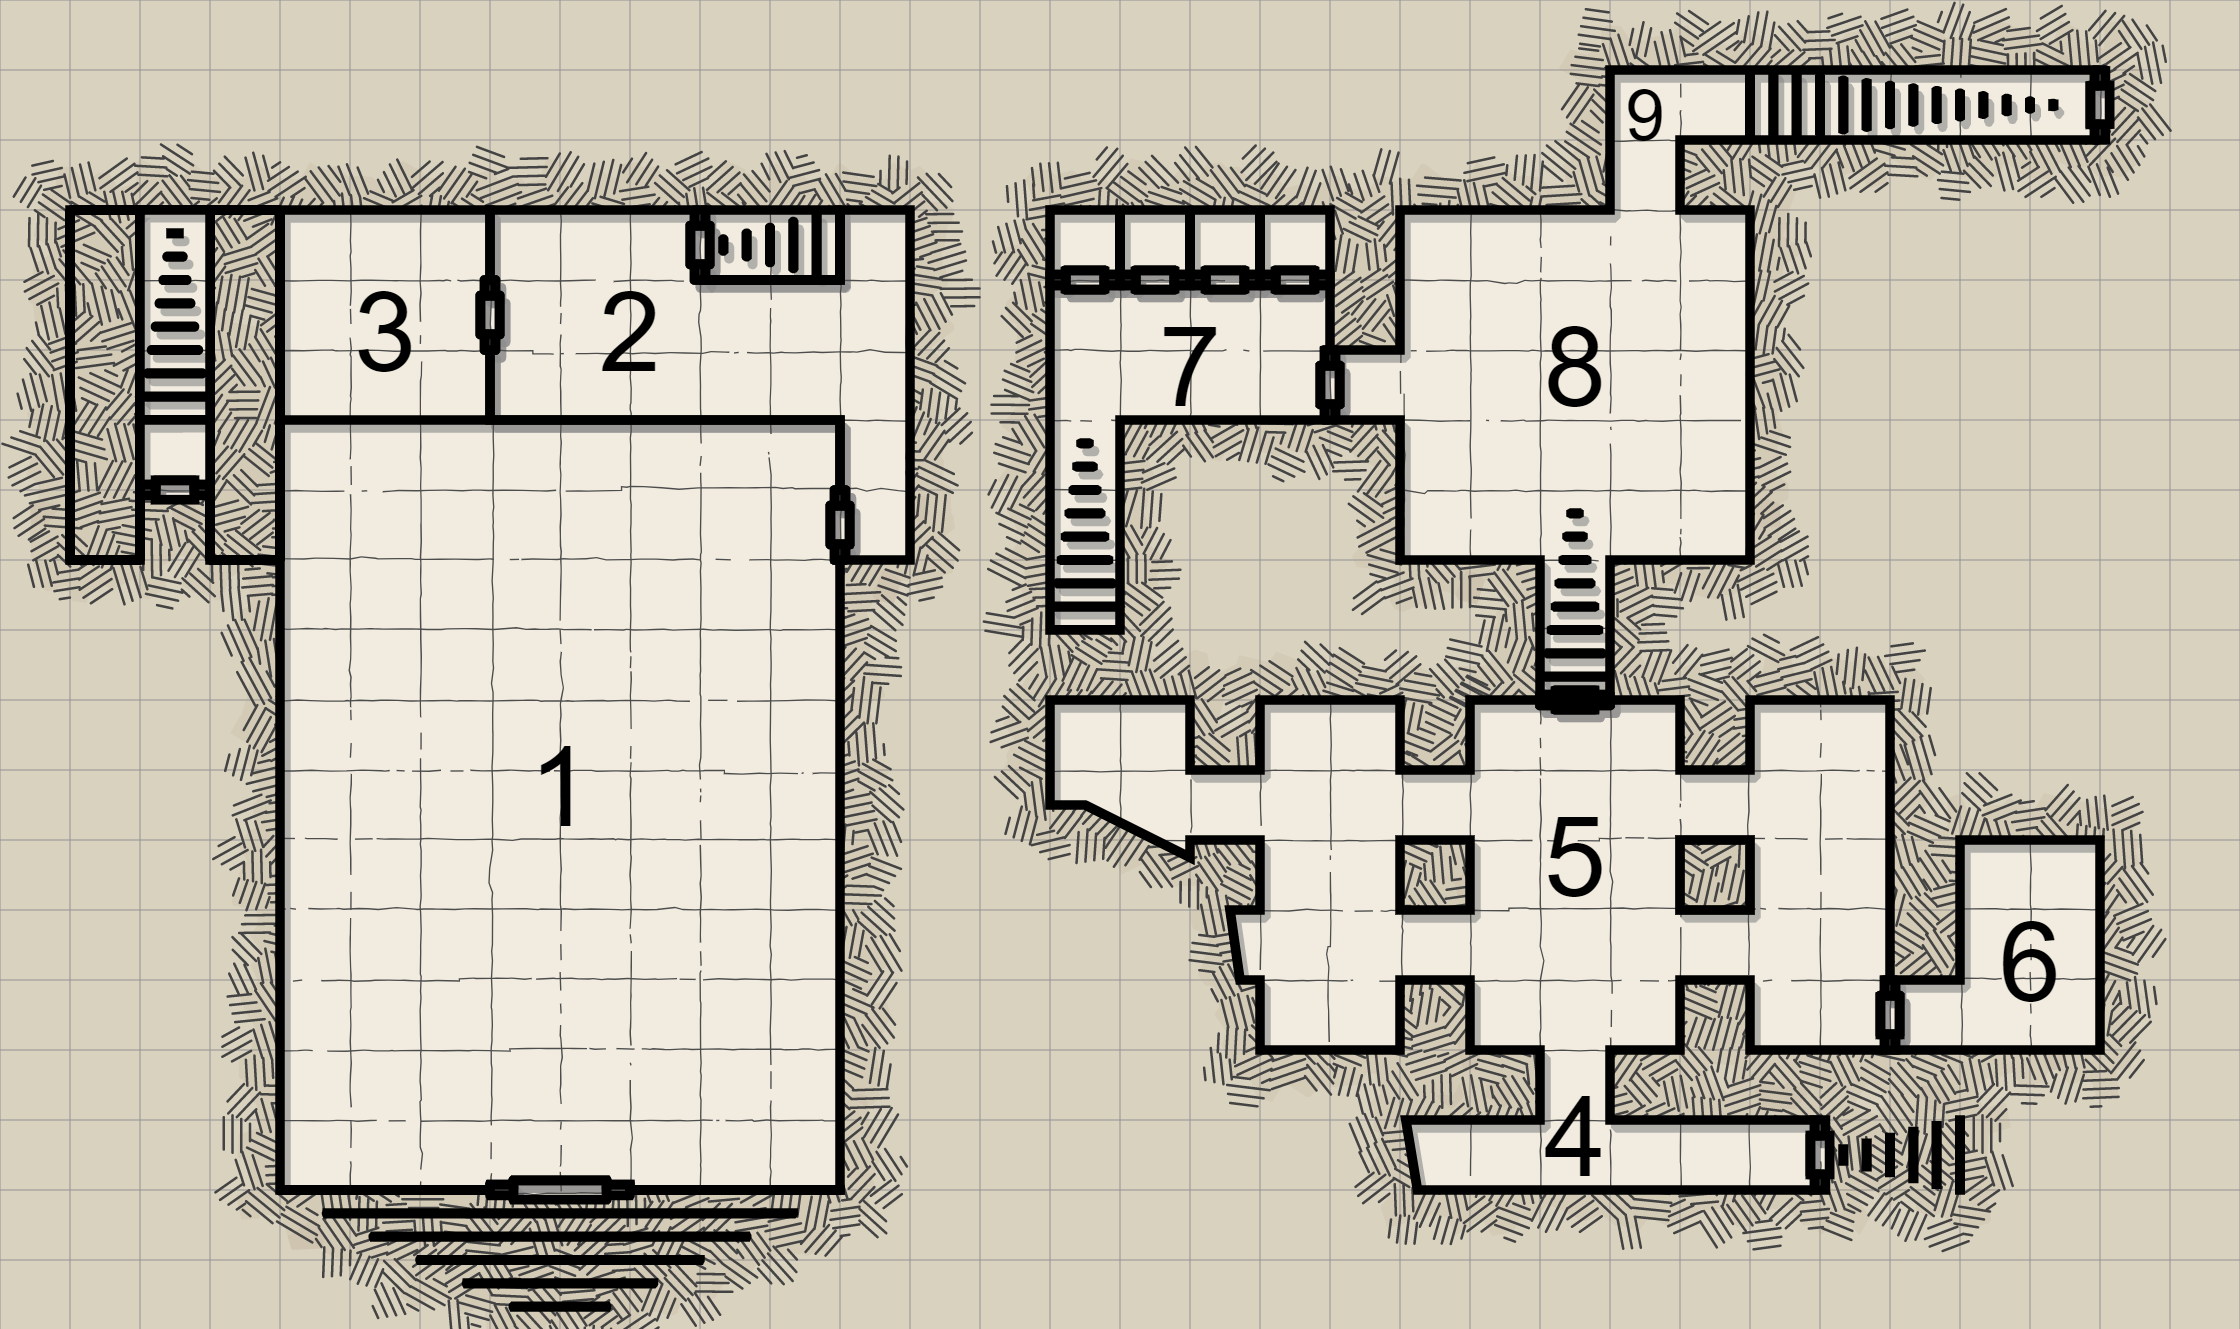
\includegraphics[width=\textwidth]{images/vaelboras_temple}
	%
\includegraphics[width=\textwidth]{images/placeholder}
	\caption{The Temple of Vael'boras with Catacombs}
\end{figure*}

\subsubsection*{\underline{1. Main Sanctuary}}
Large steps lead to double doors and the entrance to the main sanctuary of the temple. Many sculptures and stain glass windows depict various historical and mythological events related to Vael'boras theology. The sanctuary is a beautiful room where worshipers gather to listen to sermons from the high priest Laeroth. It can easily hold over a hundred people, however attendance on any given day is very sparse. The temple is open all day for worshipers and visitors and closes at sunset. 

 Steps lead to an elevated platform where Laeroth delivers is daily morning sermons and prayers. Laeroth can be found here during his sermons or during the day when people require his services. A door on the back side of the platform leads to the preparation room.
 
 There is also a secret entrance to the catacombs on the western side of the temple. The entrance is appears boarded up and covered in weeds and branches but on closer inspection and removing the obstruction reveals a locked door. The door can be picked or if Laeroth's key chain has been acquired can be unlocked. The door opens to a long staircase leading down to \textbf{area 7}. This is the entrance used by Laeroth and the children of Abruhan to smuggle in people that have been abducted.

\subsubsection*{\underline{2. Preparation Room}}
The preparation room is used by Laeroth to prepare before sermons. The room contains various religious artifacts, hymnal books, and clothes used for each service, nothing of real value or interest. A permanently locked door is found on the other side of the room leading to Laeroth's quarters which can be picked. 

Additionally, a veil covers the entry into the staircase leading down to the catacombs. At the bottom of the staircase stands a locked door, which can also be picked, which leads to \textbf{area 4} of the catacombs. Laeroth holds the keys to these doors if the players manage to steal them. The door is covered in cobwebs misleading players into thinking this way hasn't been used in a very long time, however, the cobwebs are actually a magical illusion meant to deter people. This can be discovered using an investigation or arcana check. 

\subsubsection*{\underline{3. Laeroth's Quarters}}
Being devoted and the primary caretaker to the temple, Laeroth's actually lives in the temple in quarters reserved for him. He spends most of his evenings in his quarters preparing his sermons and secretly studying Uhanos mythology.
 
The desk where Laeroth studies contains various books and notes, and a secret compartment (DC 15 investigation check required to discover) containing some of the books stolen from the Great Library. Included with the books are various notes taken by Laeroth detailing his motives, his direct involvement with the children of Abruhan and the abductions, his frustrations with Vael'boras, and his desires to serve and raise Uhanos as the prime deity ruling over Valboro. He ends his letters and notes with "Praise Uhanos!".

\subsubsection*{\underline{\textbf{Treasure}}}
His possessions are mostly what one would expect from someone's quarters, mainly clothes, books. Upon investigation, underneath the bed is a chest containing some of Laeroth's more valuable possessions: 280sp, 120gp, a jeweled chalice worth 150gp, two \textbf{two Potions of Healing} and an ancient scroll of Vael'boras scripture for which Erlan Qinmaer at the Great Library will gladly pay 250gp to be able to study.

\subsubsection*{\underline{4. Catacomb Entrance}}
The catacombs of the Vael'boras temple are ancient and were used  as tombs for notable kings from the past. It is not in use anymore and is rarely frequented with the exception of Laeroth and the children of Abruhan using it for rituals and for smuggling of abductees. The catacombs are dimly lit with torches and the air smells of death and rot. The entrance to the catacomb from inside the temple is a long corridor which ends in rubble that has collapsed at some point in time. A passage to the north of the corridor gives access to the main tombs. 

There is a \textbf{trap} on the floor which fires a poison dart from the ceiling support. Spotting the trap will require a DC 12 perception or investigation check. Springing the trap requires a DC 15 dexterity saving throw to avoid the dart. A failure deals 2d8 damage and poisons the target, while a success halves the damage and the target is not poisoned. This trap is used by Laeroth to ward off possible intruders. There is a switch to disable the trap hidden behind a support column on the wall which requires a DC 15 investigation check to find. If the trap is not disarmed, the players will have to perform an acrobatics check to jump over the trap to avoid it.

\subsubsection*{\underline{5. Tombs}}
The main ancient tomb where past kings have been laid to rest is a fairly large room with pillars and arches holding up the remains of the catacombs. The walls are lined with many sarcophagi containing mummified remains of past kings and priests. There is a door to the north leading to the ritual chamber, and a door in the eastern corner of the rooms, both unlocked. The western end of the chamber has collapsed in an earthquake many centuries ago. 

Many remains of people who likely died in the earthquake litter the floor, including two guards (\textbf{wights}) leaning against pillars. Among the remains, two other more recently decaying bodies (\textbf{zombie}) with poison darts sticking from their sides, can be found lying face down on the floor. The bodies are unfortunate wanderers who have ventured into the catacombs and got caught in the trap. Investigating the bodies and dead guards requires a DC 20 check to determine that they are in fact undead. A successful check will give players a surprise round for the combat. Spending too much time investigating the tomb or attempting to open the door leading to the ritual chamber will awake the two \textbf{wights} and two \textbf{zombies}.

\subsubsection*{\underline{\textbf{Treasure}}}
If the players choose to carefully investigate the sarcophagi, they will find a \textbf{Greatsword +1} (\emph{martial, two-handed, 2d6+1}) and a \textbf{Ring of Resistance} (roll for resistance type) in the sarcophagus of the great king Ganamede. Spending too much time in the tomb will awake the zombies and wights.

\subsubsection*{\underline{6. Embalming Room}}

The embalming room was used to prepare the bodies before laying them to rest. The room includes desks, shelves with various embalming tools, and a table in the center used for the bodies. The room has not be in use for centuries and has been damaged in the last earthquake. Two unharmed \textbf{skeletons} are on the floor and the remains of a \textbf{mummy} is laying on the table. Any prolonged investigation of the room wakes the skeletons and the mummy.

\subsubsection*{\underline{\textbf{Treasure}}}
On one of the shelves, two flasks of \textbf{Oil of Sharpness} can be found. An investigation check reveals that this oil has magical properties, and an arcana reveals it's magical properties.
 
\end{multicols*}


\pagebreak
